\section{Position}
	Let
	\begin{align}
		x = \ &\text{position}& \notag \\
		x_{i} = \ &\text{initial position}& \notag \\
		x_{f} = \ &\text{final position}& \notag \\
		\Delta x = \ &\text{Displacement}& \notag \\
		= \ &x_{f}-x_{i} \notag
	\end{align}
	Example:
	\begin{align}
		x_{i} = \ &+3 \ ft& \notag \\
		x_{f} = \ &+5 \ ft& \notag \\
		\Delta x = \ &x_{f} - x_{i}& \notag \\
		= \ &5 \ ft - 3 \ ft& \notag \\
		= \ &+2 \ ft& \notag
	\end{align}
	Example:
	\begin{align}
		x_{i} = \ &+5 \ ft& \notag \\
		x_{f} = \ &-1 \ ft& \notag \\
		\Delta x = \ &x_{f} - x_{i}& \notag \\
		= \ &-1 \ ft -5 \ ft& \notag \\
		= \ &-6 \ ft& \notag
	\end{align}
	Example:
	\begin{align}
		x_{i} = \ &+3 \ ft& \notag \\
		x_{2} = \ &+5 \ ft& \notag \\
		x_{f} = \ &-1 \ ft& \notag \\
		\Delta x = \ &x_{f} - x_{i}& \notag \\
		= \ &-1 \ ft - 3 \ ft& \notag \\
		= \ &-4 \ ft& \notag \\
		\text{Distance Traveled} = \ &2 \ ft + 6 \ ft& \notag \\
		= \ &8 \ ft& \notag
	\end{align}

\section{Velocity}
	\begin{align}
		\bar{v} = \ &\text{average velocity}& \notag \\
		\bar{v} \equiv \ &\frac{\Delta x}{\Delta t} = \frac{\text{displacement}}{\text{time elapsed}}& \notag \\
		\text{average speed} = \ &\frac{\text{distance travelled}}{\text{time elapsed}}& \notag
	\end{align}
	Example:
	\begin{align}
		\text{Start at } x = \ &+3 \ ft& \notag \\
		\text{Move to } x = \ &+5 \ ft& \notag \\
		\text{End at } x = \ &-1 \ ft& \notag \\
		\text{Trip takes } &4 \ s& \notag \\
		\text{Find } &a) average velocity& \notag \\
		&b) average speed& \notag
	\end{align}
	\begin{align}
		\bar{v} \equiv \ &\frac{\Delta x}{\Delta t}& \notag \\
		= \ &\frac{-1 \ ft - 3 \ ft}{4 \ s} = \frac{-4 \ ft}{4 \ s} = -1 \ ft/s& \notag \\
		\text{average speed} = \ &\frac{\text{distance}}{\text{time}} = \frac{8 \ ft}{4 \ s} = 2 \ ft/s& \notag
	\end{align}

	\begin{figure}[H]
		\begin{center}
			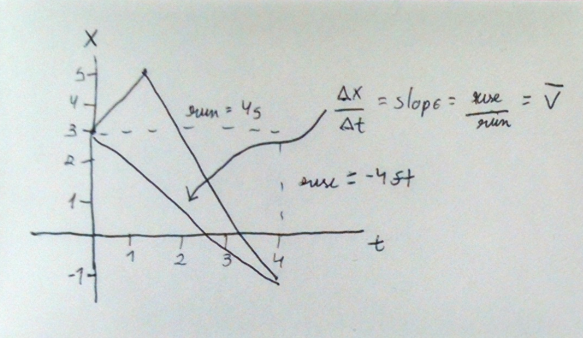
\includegraphics[scale=0.43]{01_25_01}
			\caption{Graphic of the Average Speed}
			\label{fig:01_25_01}
		\end{center}
	\end{figure}

	\begin{align}
		v = \ &\text{instantaneous velocity}& \notag \\
		= \ &\lim_{\Delta t \to 0} \frac{\Delta x}{\Delta t}& \notag \\
		v \equiv \ &\frac{dx}{dt}& \notag
	\end{align}
	Example:
	\begin{align}
		x = \ &3 \ m + (17 \ m/s)t + (7 \ m/s^{3})t^{3}& \notag \\
		\text{Find} && \notag \\
		&a) \text{position at } t = 2 \ s& \notag \\
		&b) \text{position at } t = 4 \ s& \notag \\
		&c) \text{average velocity from} 2 \ s \to 4 \ s& \notag
	\end{align}
	a)
	\begin{align}
		x = \ &3 \ m + (17 \ m/s)(2 \ s) + (7 \ m/s^{3})(2 \ s)^{3}& \notag \\
		= \ &3 \ m + 34 \ m + 56 \ m& \notag \\
		= \ &93 \ m& \notag \\
	\end{align}
	b)
	\begin{align}
		x = \ &3 \ m + (17 \ m/s)(4 \ s) + (7 \ m/s^{3})(4 \ s)^{3}& \notag \\
		= \ &3 \ m + 68 \ m + 448 \ m& \notag \\
		= \ &519 \ m& \notag
	\end{align}
	c)
	\begin{align}
		\bar{v} = \ &\frac{\Delta x}{\Delta t} = \frac{519 \ m - 93 \ m}{4 \ s - 2 \ s}& \notag \\
		= \ &\frac{426 \ m}{2 \ s}& \notag \\
		= \ &213 \ m/s& \notag
	\end{align}
	d)
	\begin{align}
		v = \ &\frac{dx}{dt}& \notag \\
		= \ &\frac{d}{dt}\left[ 3 \ m + (17 \ m/s)t + (7 \ m/s^{3})t^{3} \right] \notag \\
		= \ &0 + 17 \ m/s + (21 \ m/s^{3})t^{2}& \notag \\
		v(3 \ s) = \ &17 \ m/s + (21 \ m/s^{3})(3 \ s)^{2}& \notag \\
		= \ &17 \ m/s + 189 \ m/s = 208 \ m/s& \notag
	\end{align}

	\begin{figure}[H]
		\begin{center}
			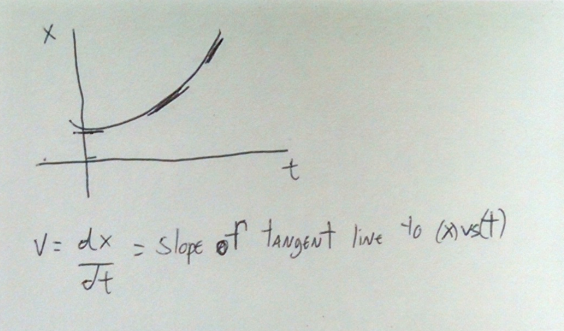
\includegraphics[scale=0.43]{01_25_02}
			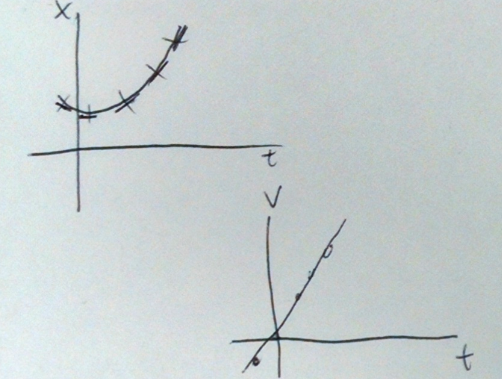
\includegraphics[scale=0.43]{01_25_03}
			\caption{Graphics of Instantaneous Velocity}
			\label{fig:01_25_02-03}
		\end{center}
	\end{figure}
